\documentclass{ximera}


\graphicspath{
  {./}
  {ximeraTutorial/}
  {basicPhilosophy/}
}

\newcommand{\mooculus}{\textsf{\textbf{MOOC}\textnormal{\textsf{ULUS}}}}


\usepackage{tkz-euclide}\usepackage{tikz}
\usepackage{tikz-cd}
\usetikzlibrary{arrows}
\tikzset{>=stealth,commutative diagrams/.cd,
  arrow style=tikz,diagrams={>=stealth}} %% cool arrow head
\tikzset{shorten <>/.style={ shorten >=#1, shorten <=#1 } } %% allows shorter vectors

\usetikzlibrary{backgrounds} %% for boxes around graphs
\usetikzlibrary{shapes,positioning}  %% Clouds and stars
\usetikzlibrary{matrix} %% for matrix
\usepgfplotslibrary{polar} %% for polar plots
\usepgfplotslibrary{fillbetween} %% to shade area between curves in TikZ
\usetkzobj{all}
\usepackage[makeroom]{cancel} %% for strike outs
%\usepackage{mathtools} %% for pretty underbrace % Breaks Ximera
%\usepackage{multicol}
\usepackage{pgffor} %% required for integral for loops



%% http://tex.stackexchange.com/questions/66490/drawing-a-tikz-arc-specifying-the-center
%% Draws beach ball
\tikzset{pics/carc/.style args={#1:#2:#3}{code={\draw[pic actions] (#1:#3) arc(#1:#2:#3);}}}



\usepackage{array}
\setlength{\extrarowheight}{+.1cm}
\newdimen\digitwidth
\settowidth\digitwidth{9}
\def\divrule#1#2{
\noalign{\moveright#1\digitwidth
\vbox{\hrule width#2\digitwidth}}}
























%%This is to help with formatting on future title pages.
\newenvironment{sectionOutcomes}{}{}


\title{Right Triangles}

\begin{document}

\begin{abstract}
%%%
\end{abstract}
\maketitle


Every triangle can be divided into two right triangles.









\begin{image}[3in]
    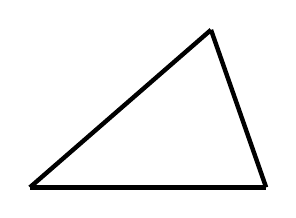
\begin{tikzpicture}

  %\draw [ultra thick] (0,0) -- (0,3);
  \draw [ultra thick] (0,0) -- (3,0);
  \draw [ultra thick] (3,0) -- (2.3,2);
  %\draw [ultra thick] (0,3) -- (3,3);

 
  \draw [ultra thick] (0,0) -- (2.3,2);



    \end{tikzpicture}
  \end{image}




























\begin{image}[3in]
    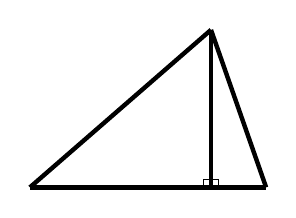
\begin{tikzpicture}

  %\draw [ultra thick] (0,0) -- (0,3);
  \draw [ultra thick] (0,0) -- (3,0);
  \draw [ultra thick] (3,0) -- (2.3,2);
  %\draw [ultra thick] (0,3) -- (3,3);

 
  \draw [ultra thick] (0,0) -- (2.3,2);
  \draw [ultra thick] (2.3,0) -- (2.3,2);


  \draw [thin] (2.2,0.10) -- (2.4, 0.10);
  \draw [thin] (2.2,0) -- (2.2,0.10);
  \draw [thin] (2.4,0) -- (2.4,0.10);



    \end{tikzpicture}
  \end{image}




If we can understand right triangles, then we can understand any triangle.










\subsection{Learning Outcomes}


\begin{sectionOutcomes}
In this section, students will 

\begin{itemize}
\item study right triangles.
\item study general triangles.
\end{itemize}
\end{sectionOutcomes}

\end{document}
